\documentclass{article}
\usepackage{amsmath}
\usepackage{amssymb}
\usepackage[svgnames]{xcolor}
\usepackage{graphicx}
\usepackage{enumitem}
\usepackage{multicol}
\usepackage{graphicx}
\usepackage{color}


\begin{document}
\section{Sum-product Algorithm}
\begin{figure}[htb!]
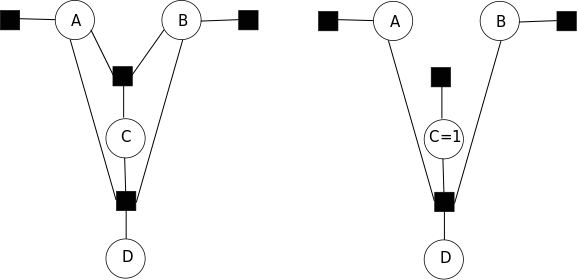
\includegraphics[width = \textwidth]{ex01.png}
\end{figure}

The graph is now in tree structure, acyclic.
\begin{table}[htb]
\caption{$f_A$}
\centering
  \begin{tabular}{ | c | c | c | c | c | c | c | c |}
    \hline
    A & B & C & D & $f_A$ & $f_B$ & $f_C$ & $f_D$ \\ \hline
    1 & 1 & 1 & 1 & 1 & 1 & 1 & 1\\\hline
    0 & 0 & 1 & 0 & 0 & 0 & 0 & 1\\\hline
    1 & 0 & 1 & 0 & 1 & 0 & 1 & 1\\\hline
    0 & 1 & 1 & 0 & 0 & 1 & 1 & 0\\\hline
	0 & 0 & 1 & 1 & 0 & 0 & 0 & 0\\\hline
	1 & 1 & 1 & 0 & 0 & 0 & 0 & 0\\\hline
	1 & 0 & 1 & 1 & 0 & 0 & 0 & 0\\\hline
	0 & 1 & 1 & 1 & 0 & 0 & 0 & 0\\\hline

  \end{tabular}
\end{table}



\end{document}